\documentclass[12pt,border=0pt]{standalone}

\usepackage[utf8]{inputenc} 
\usepackage{amssymb,amsmath}
\usepackage{tikz}
\usetikzlibrary{shapes}

\definecolor{aliceblue}{rgb}{0.94, 0.97, 1.0}
\definecolor{aquamarine}{rgb}{0.5, 1.0, 0.83}


\thispagestyle{empty}

\begin{document}

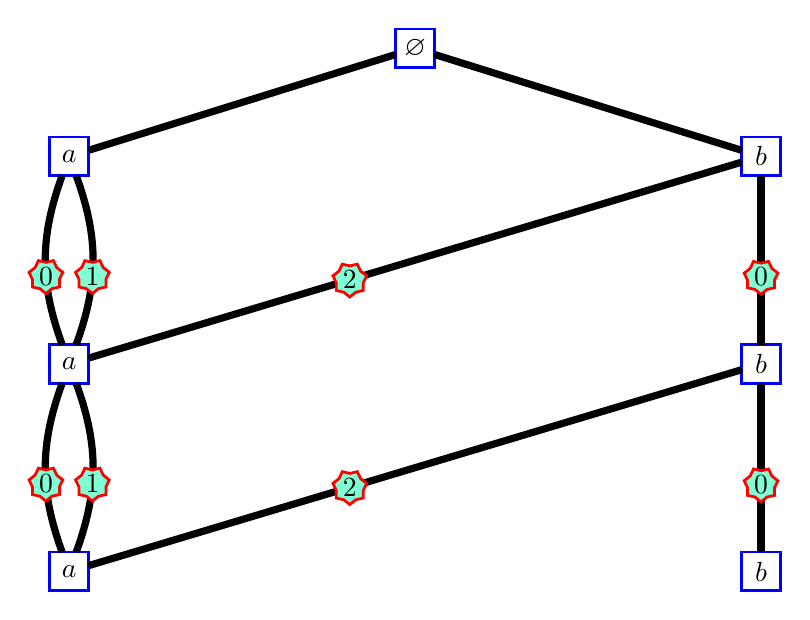
\begin{tikzpicture}[x=10pt,y=6pt]
  \centering
  \tikzset{VertexStyle/.style = {
    shape         = rectangle,
    draw          = blue, 
    fill          = white, 
  	line width    = 1pt, 
    text          = black,
    inner sep     = 1pt,
    outer sep     = 0pt,
    minimum size  = 14 pt,
    scale         = 1
    }
  }
  \tikzset{EdgeStyle/.style = {
    draw            = black, 
    thick,
    double          = black,
    double distance = 1pt
    }
  }
  \tikzset{EdgeLabelStyle/.style = {
    draw          = red,
  	shape         = star,star points=7,star point ratio=0.8,
  	line width    = 1pt, 
  	minimum size  = 10pt, 
    inner sep     = 1pt,
    outer sep     = 0pt,
    fill          = aquamarine,
    text          = black,
    scale         = 1,
    pos = 0.6
    }
  }

	\node[VertexStyle](A1) at (25, 37.75) {$\varnothing$};
	\node[VertexStyle](B1) at (12.5, 31.25) {$a$};
	\node[VertexStyle](B2) at (37.5, 31.25) {$b$};
	\node[VertexStyle](C1) at (12.5, 18.75) {$a$};
	\node[VertexStyle](C2) at (37.5, 18.75) {$b$};
	\node[VertexStyle](D1) at (12.5, 6.25) {$a$};
	\node[VertexStyle](D2) at (37.5, 6.25) {$b$};
	\draw[EdgeStyle](A1) to (B1);
	\draw[EdgeStyle](A1) to (B2);
	\draw[EdgeStyle, bend left=-20](B1) to node[EdgeLabelStyle]{$0$} (C1);
	\draw[EdgeStyle, bend left=20](B1) to node[EdgeLabelStyle]{$1$} (C1);
	\draw[EdgeStyle](B2) to node[EdgeLabelStyle]{$2$} (C1);
	\draw[EdgeStyle](B2) to node[EdgeLabelStyle]{$0$} (C2);
	\draw[EdgeStyle, bend left=-20](C1) to node[EdgeLabelStyle]{$0$} (D1);
	\draw[EdgeStyle, bend left=20](C1) to node[EdgeLabelStyle]{$1$} (D1);
	\draw[EdgeStyle](C2) to node[EdgeLabelStyle]{$2$} (D1);
	\draw[EdgeStyle](C2) to node[EdgeLabelStyle]{$0$} (D2);

  \end{tikzpicture}

\end{document}
